% !TeX root = ../libro.tex
% !TeX encoding = utf8

\chapter{Ejemplo extendido de cálculo de geodésicas con BFS}\label{ap:apendice1}

Con afán de mostrar el procedimiento del algoritmo BFS sobre un grafo de mayor extensión, se presenta a continuación en la \autoref{fig:bfs-camino-big} el proceso de búsqueda de geodésicas, donde cada imagen representa el estado del grafo al finalizar una capa, es decir, tras explorar por completo cada bola, el nodo inicial es el nodo $0$, y el nodo final está marcado en rojo para mejor visibilidad. Los nodos ya explorados se han marcado en verde oscuro, y los nodos visitados pero no explorados, es decir, los nodos en la cola, en verde pistacho. Los caminos marcados en rojo representan las geodésicas encontradas, que se pueden calcular a través de los predecesores de cada nodo.

\begin{figure}[htb]
	\centering
	\begin{subfigure}{0.28\linewidth}
		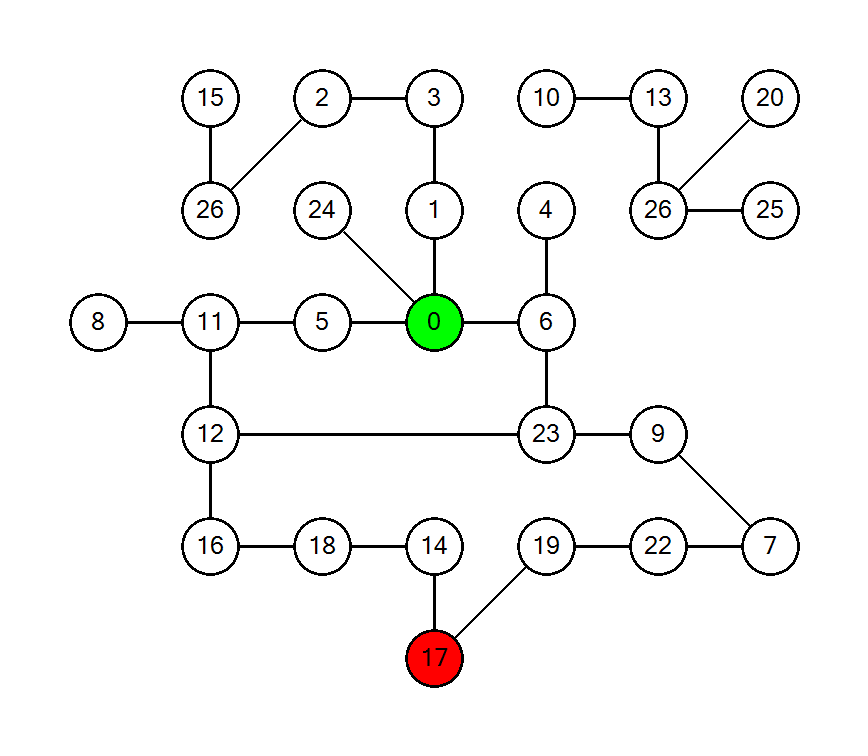
\includegraphics[width=\linewidth]{BFS/graf-bfs-camino-big-1}
		\caption{}
	\end{subfigure}
	\begin{subfigure}{0.28\linewidth}
		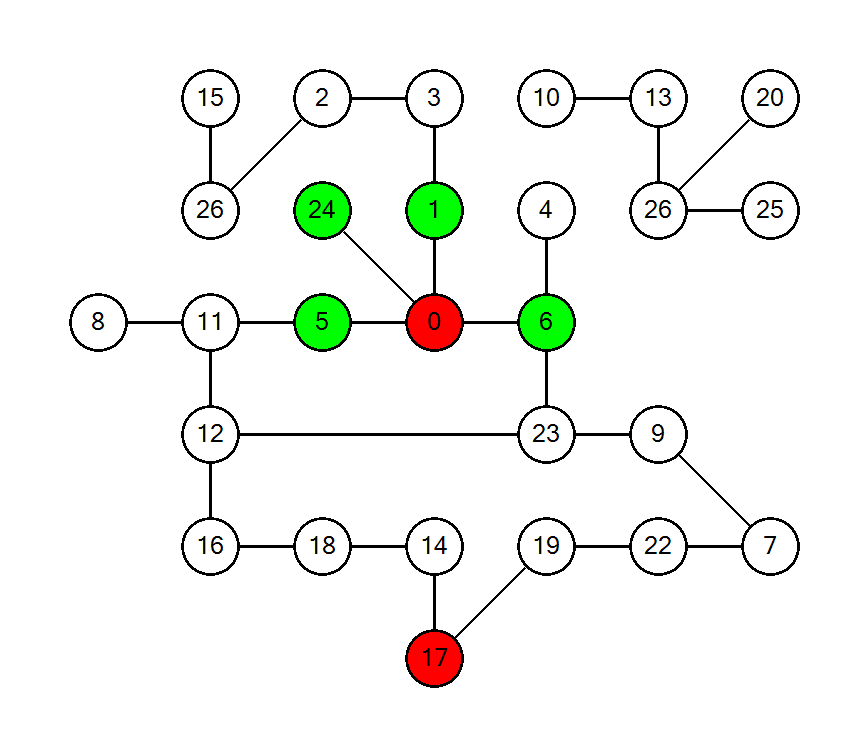
\includegraphics[width=\linewidth]{BFS/graf-bfs-camino-big-2}
		\caption{}
	\end{subfigure}
	\begin{subfigure}{0.28\linewidth}
		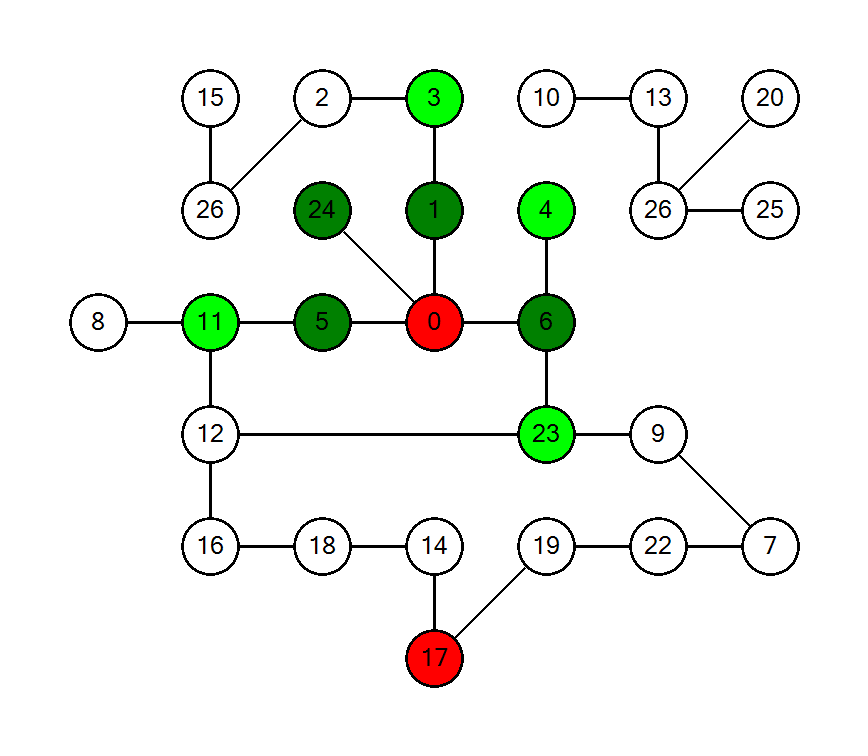
\includegraphics[width=\linewidth]{BFS/graf-bfs-camino-big-3}
		\caption{}
	\end{subfigure}
	\begin{subfigure}{0.28\linewidth}
		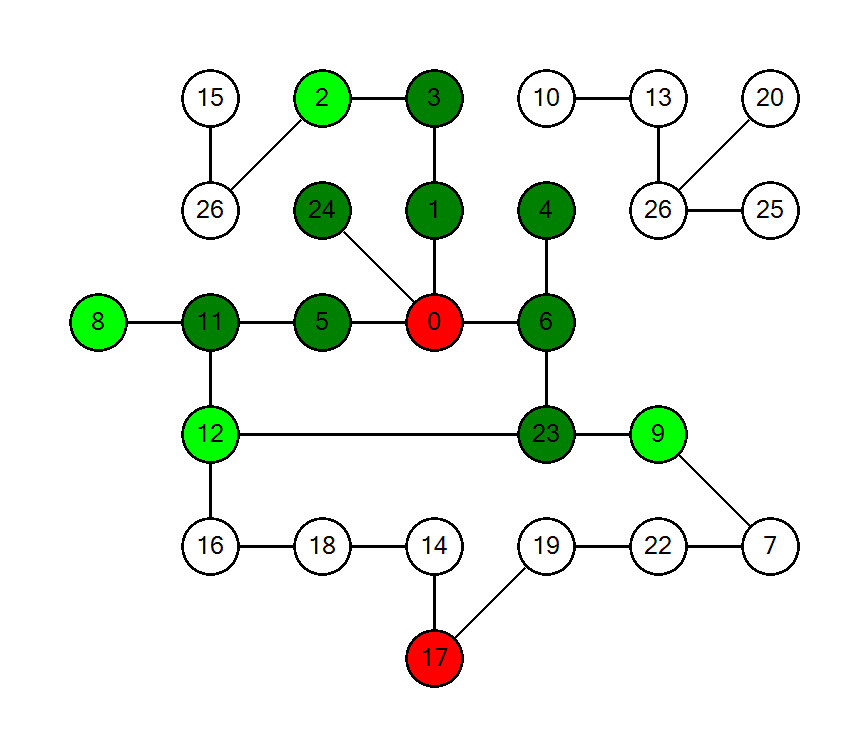
\includegraphics[width=\linewidth]{BFS/graf-bfs-camino-big-4}
		\caption{}
	\end{subfigure}
	\begin{subfigure}{0.28\linewidth}
		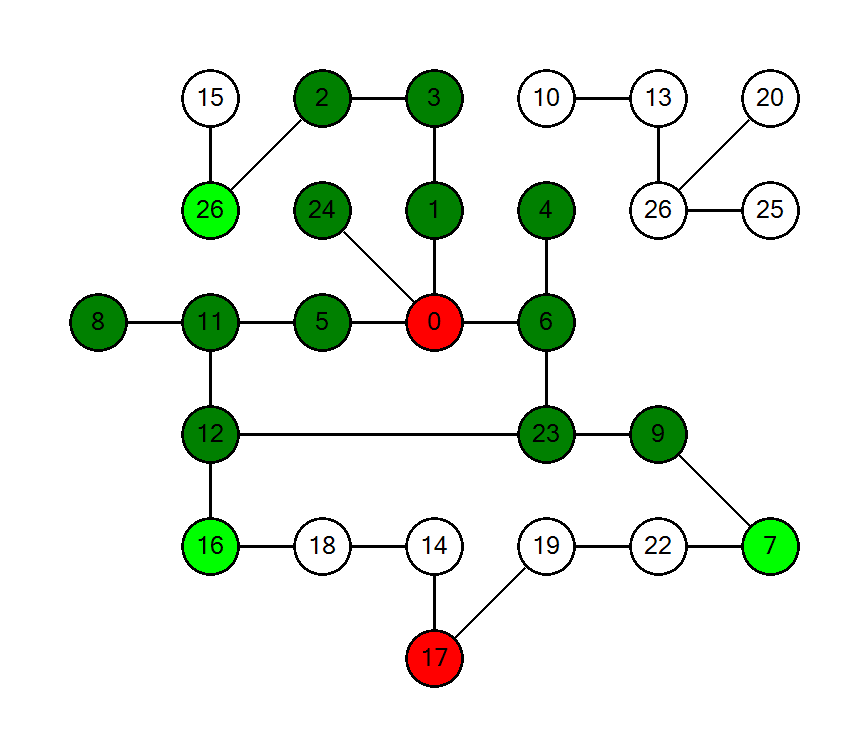
\includegraphics[width=\linewidth]{BFS/graf-bfs-camino-big-5}
		\caption{}
	\end{subfigure}
	\begin{subfigure}{0.28\linewidth}
		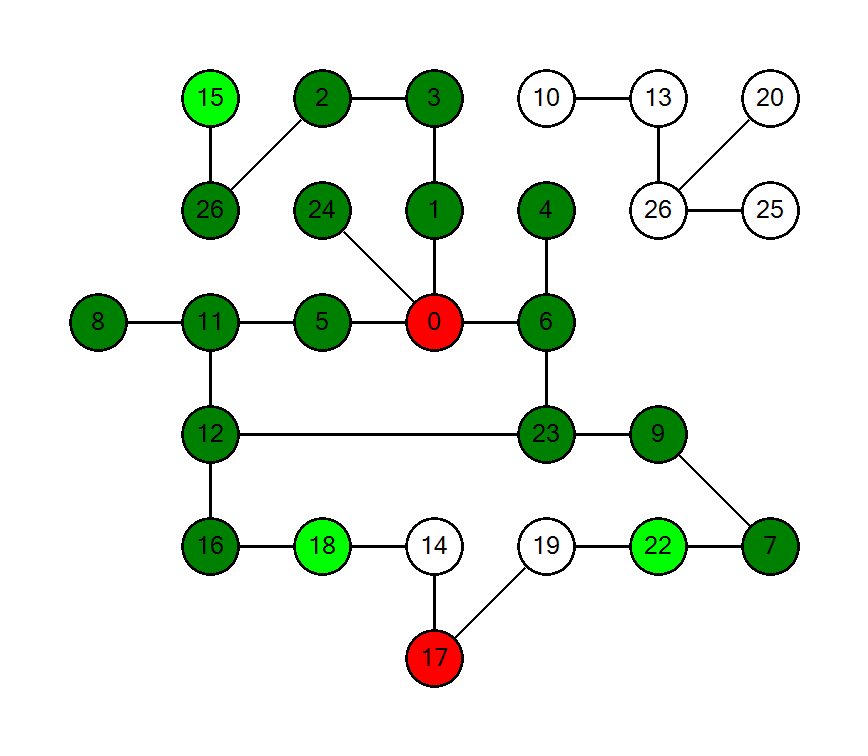
\includegraphics[width=\linewidth]{BFS/graf-bfs-camino-big-6}
		\caption{}
	\end{subfigure}
	\begin{subfigure}{0.28\linewidth}
		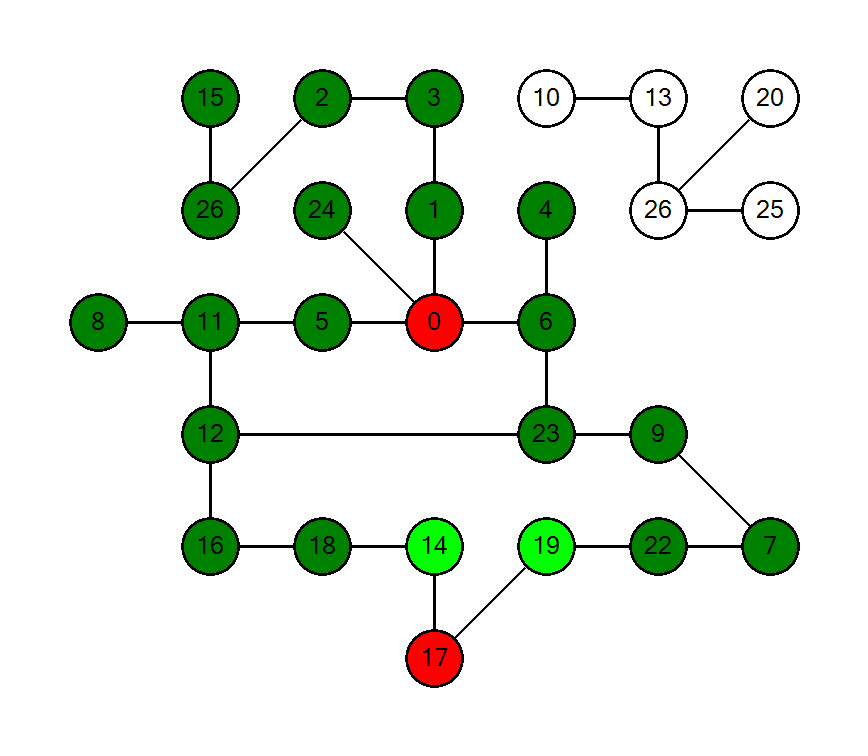
\includegraphics[width=\linewidth]{BFS/graf-bfs-camino-big-7}
		\caption{}
	\end{subfigure}
	\begin{subfigure}{0.28\linewidth}
		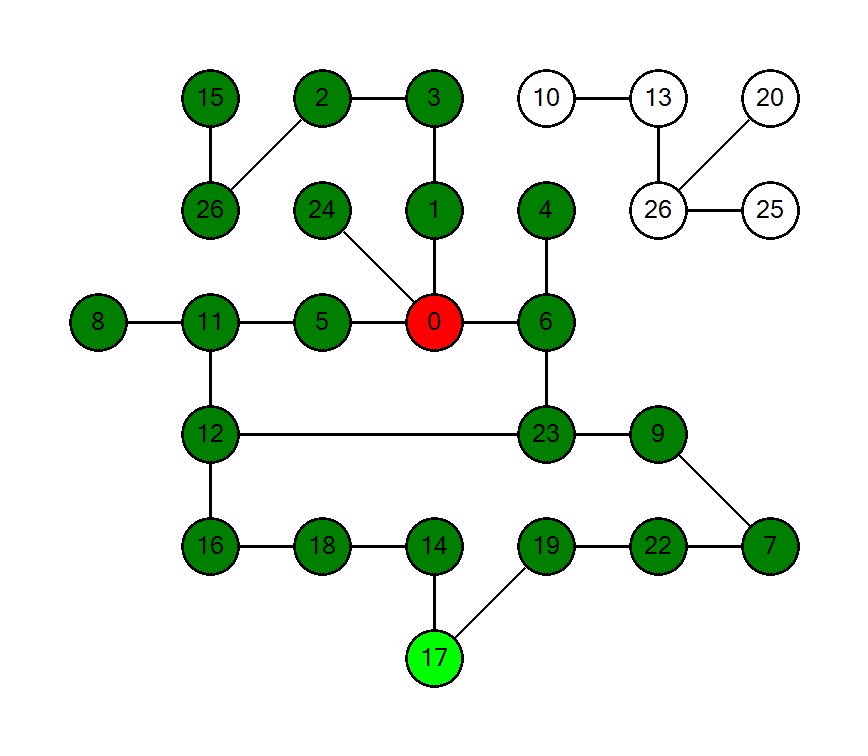
\includegraphics[width=\linewidth]{BFS/graf-bfs-camino-big-8}
		\caption{}
	\end{subfigure}
	\begin{subfigure}{0.28\linewidth}
		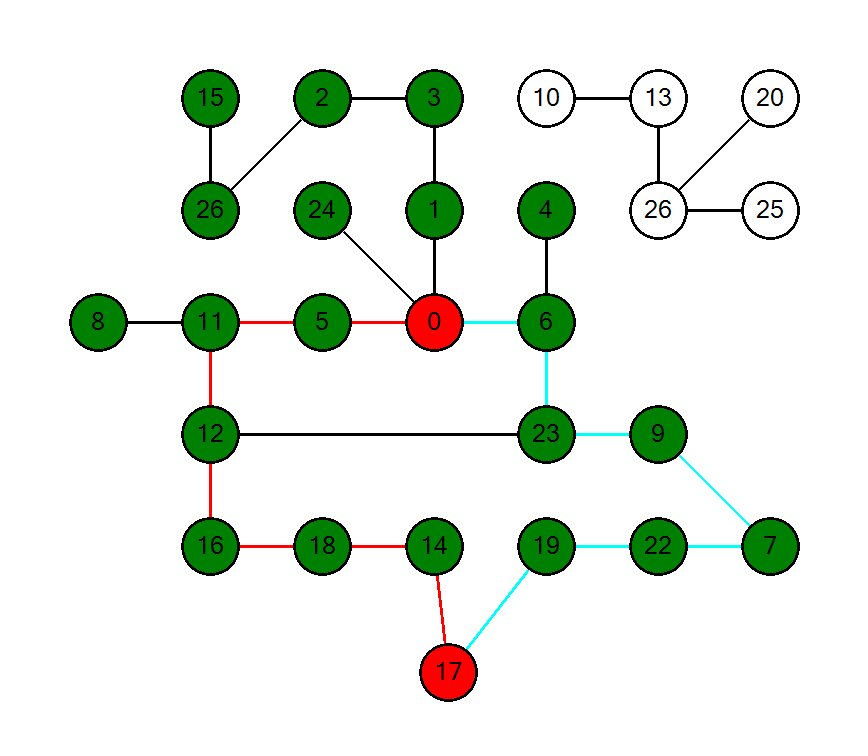
\includegraphics[width=\linewidth]{BFS/graf-bfs-camino-big-9}
		\caption{}
	\end{subfigure}
	\caption{Cálculo de las geodésicas entre el nodo $0$ y el nodo $17$, marcado en rojo.}
	\label{fig:bfs-camino-big}
\end{figure}


\endinput
%------------------------------------------------------------------------------------
% FIN DEL APÉNDICE. 
%------------------------------------------------------------------------------------
